\subsection{The Process Life Cycle}\label{subsec:Process_Life_Cycle}
A \nameref{def:Process} begins its life when, the \kernelinline{fork()} \nameref{def:System_Call} is called.
This creates a new \nameref{def:Process} by duplicating an existing one.
The \nameref{def:Process} that calls \kernelinline{fork()} is the \textbf{parent}, whereas the new \nameref{def:Process} is the \textbf{child}.
The \kernelinline{fork()} \nameref{def:System_Call} returns from the kernel twice: once in the \textbf{parent} and once in the newborn \textbf{child}.
The parent resumes execution and the child starts execution at the same place, where the call to \kernelinline{fork()} returns.

Often, immediately after a \texttt{fork} it is desirable to execute a new, different \nameref{def:Program}.
The \kernelinline{exec()} family of function calls creates a new address space and loads a new program into it.

Finally, a program exits via the \kernelinline{exit()} \nameref{def:System_Call}.
This function terminates the \nameref{def:Process} and frees all its resources.
A parent \nameref{def:Process} can inquire about the status of a terminated child via the \kernelinline{wait4()} \nameref{def:System_Call}, which enables a \nameref{def:Process} to wait for the termination of a specific \nameref{def:Process}.
When a \nameref{def:Process} exits, it is placed into a special zombie state that represents terminated \nameref{def:Process}es until the parent calls \kernelinline{wait()} or \kernelinline{waitpid()}.

\subsubsection{Process States}\label{subsubsec:Process_States}
Every \nameref{def:Process} exists in a state that describes how the process can and will behave.
\begin{itemize}[noitemsep]
\item \textbf{New}: The process is in the stage of being created.
\item \textbf{Ready}: The process has all the resources available that it needs to run, but the CPU is not currently working on this process's instructions.
\item \textbf{Running}: The CPU is working on this process's instructions.
\item \textbf{Waiting}: The process cannot run at the moment, because it is waiting for some resource to become available or for some event to occur.
\item \textbf{Terminated}: The process has completed.
\end{itemize}

\begin{figure}[h!tbp]
  \centering
  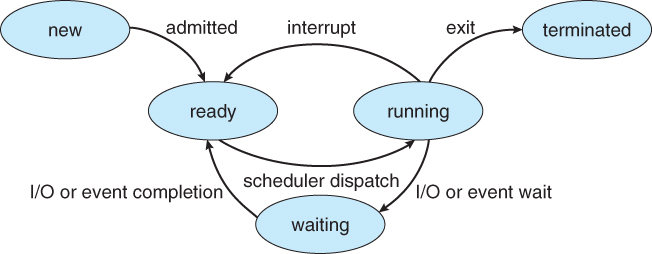
\includegraphics[scale=0.85]{./Drawings/EDAF35-Operating_Systems/Process_Life_Cycle.jpg}
  \caption{Process Life Cycle}
  \label{fig:Process_Life_Cycle}
\end{figure}

\subsubsection{Process Control Blocks and Context Switching}\label{subsubsec:PCBs_Context_Switching}
The information that is saved during a \nameref{def:Context_Switch} (An example is shown in \Cref{fig:Context_Switch}) is saved in the \nameref{def:Process_Control_Block}.

\begin{definition}[Context Switch]\label{def:Context_Switch}
  A \emph{context switch} is performed when a computer is performing several different \nameref{def:Process}es in sequence.
  A context switch involves saving the state of the currently running \nameref{def:Process} into a \nameref{def:Process_Control_Block}, and then loading a waiting process from its \nameref{def:Process_Control_Block}.
  After saving the information, every register in the CPU has its values changes to the new control blocks values, and the CPU continues execution.

  A visualization of a context switch is shown in \Cref{fig:Context_Switch}.
\end{definition}

\begin{figure}[h!tbp]
  \centering
  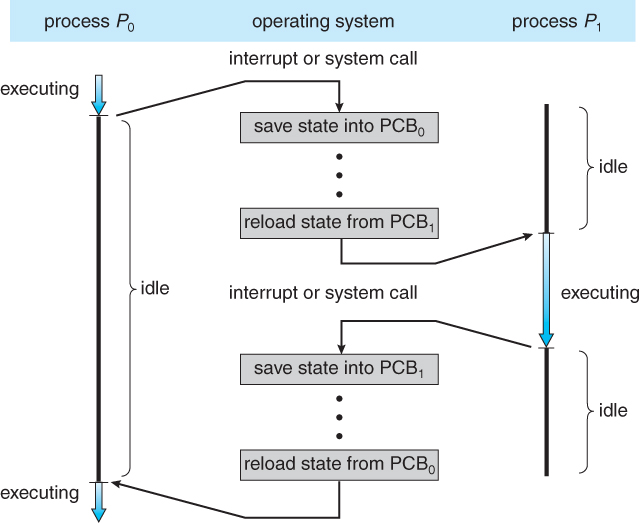
\includegraphics[scale=0.85]{./Drawings/EDAF35-Operating_Systems/Context_Switch.jpg}
  \caption{Diagram of a Context Switch}
  \label{fig:Context_Switch}
\end{figure}

\begin{definition}[Process Control Block]\label{def:Process_Control_Block}
  The \emph{process control block} (\emph{PCB}) contains \textbf{ALL} the state information (the processor's context) needed for a CPU to perform a context switch, either because of \nameref{def:Preemption} or because the process terminated.
  The information that the PCB contains includes:
  \begin{itemize}[noitemsep]
  \item Process State: Running, waiting, etc., as discussed in \Cref{subsubsec:Process_States}
  \item Process ID (PID), and parent process ID (PPID).\@
  \item CPU registers and Program Counter: Saved and restored when swapping processes in and out of the CPU.\@
  \item CPU-Scheduling information: Priority information and pointers to scheduling queues.
  \item Memory-Management information: Page tables or segment tables.
  \item Accounting information: \nameref{def:User} and \nameref{def:Kernel} CPU time consumed, account numbers, limits, etc.
  \item I/O Status information: Devices allocated, open file tables, etc.
  \end{itemize}
\end{definition}

\begin{figure}[h!tbp]
  \centering
  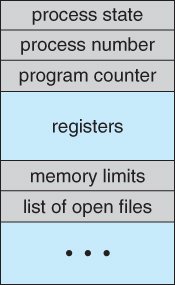
\includegraphics[scale=0.85]{./Drawings/EDAF35-Operating_Systems/Process_Control_Block.jpg}
  \caption{Process Control Block}
  \label{fig:Process_Control_Block}
  \begin{remark*}
    In \Cref{fig:Process_Control_Block}, the Process Number field is the PID of the \nameref{def:Process}.
  \end{remark*}
\end{figure}

The time spent performing a context-switch is pure overhead, because the system does no useful work while switching.
Switching speed varies from machine to machine, depending on the memory speed, the number of registers that must be copied, and the existence of special instructions (a single instruction to load or store all registers).
A typical speed is a few milliseconds.
Context-switch times are also highly dependent on hardware support.

The more complex the operating system, the greater the amount of work that must be done during a context switch.
In addition, advanced memory-management techniques may require that extra data be switched with each context.
For instance, the address space of the current process must be preserved as the space of the next task is prepared for use.

%%% Local Variables:
%%% mode: latex
%%% TeX-master: "../../EDAF35-Operating_Systems-Reference_Sheet"
%%% End:
